\documentclass{standalone}
\usepackage{tikz}
\usepackage{pgfplots}
\pgfplotsset{compat=1.18}

\begin{document}
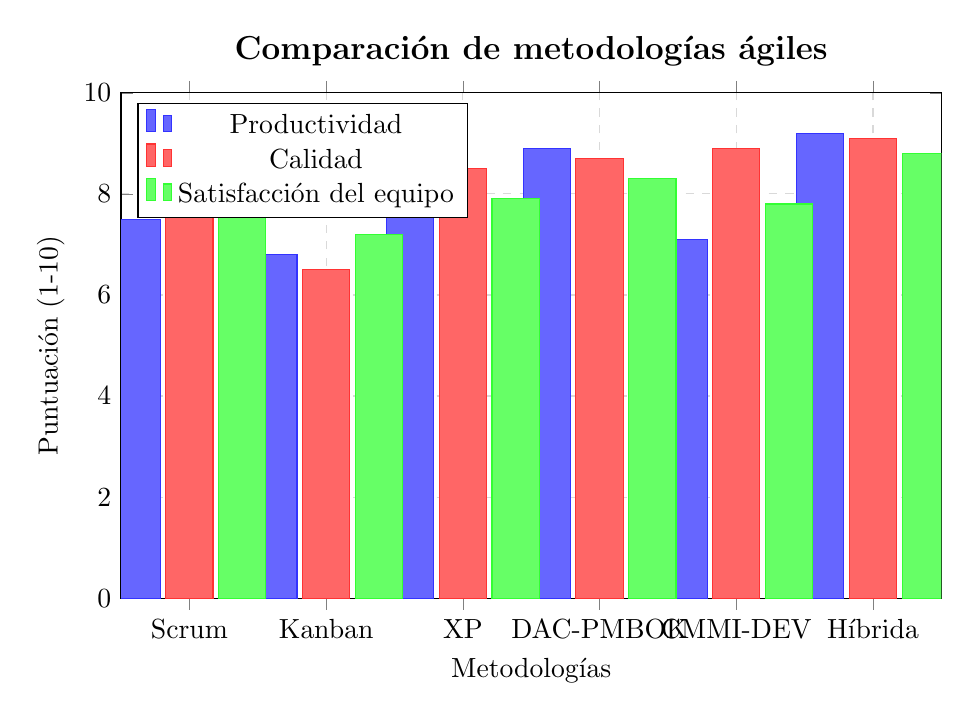
\begin{tikzpicture}
\begin{axis}[
    ybar,
    bar width=0.6cm,
    width=12cm,
    height=8cm,
    ylabel={Puntuación (1-10)},
    xlabel={Metodologías},
    xtick=data,
    xticklabels={Scrum, Kanban, XP, DAC-PMBOK, CMMI-DEV, Híbrida},
    ymin=0,
    ymax=10,
    grid=major,
    grid style={dashed,gray!30},
    legend pos=north west,
    legend style={at={(0.02,0.98)},anchor=north west},
    title={Comparación de metodologías ágiles},
    title style={font=\large\bfseries}
]

% Productividad
\addplot[fill=blue!60, draw=blue!80] coordinates {
    (1, 7.5) (2, 6.8) (3, 8.2) (4, 8.9) (5, 7.1) (6, 9.2)
};

% Calidad
\addplot[fill=red!60, draw=red!80] coordinates {
    (1, 7.8) (2, 6.5) (3, 8.5) (4, 8.7) (5, 8.9) (6, 9.1)
};

% Satisfacción del equipo
\addplot[fill=green!60, draw=green!80] coordinates {
    (1, 8.1) (2, 7.2) (3, 7.9) (4, 8.3) (5, 7.8) (6, 8.8)
};

\legend{Productividad, Calidad, Satisfacción del equipo}

\end{axis}
\end{tikzpicture}
\end{document}
